\documentclass[11pt]{article}
% NOTE: Add in the relevant information to the commands below; or, if you'll be using the same information frequently, add these commands at the top of paolo-pset.tex file. 
\newcommand{\name}{Agustín Esteva}
\newcommand{\email}{aesteva@uchicago.edu}
\newcommand{\classnum}{207}
\newcommand{\subject}{Honors Analysis in $\bbR^n$}
\newcommand{\instructors}{Luis Silvestre}
\newcommand[InternetShortcut]
URL=https://math.uchicago.edu/~may/REU2024/REUPapers/Esteva.pdf
{\assignment}{Problem Set 2}
\newcommand{\semester}{Fall 2024}
\newcommand{\duedate}{2024-14-10}
\newcommand{\bA}{\mathbf{A}}
\newcommand{\bB}{\mathbf{B}}
\newcommand{\bC}{\mathbf{C}}
\newcommand{\bD}{\mathbf{D}}
\newcommand{\bE}{\mathbf{E}}
\newcommand{\bF}{\mathbf{F}}
\newcommand{\bG}{\mathbf{G}}
\newcommand{\bH}{\mathbf{H}}
\newcommand{\bI}{\mathbf{I}}
\newcommand{\bJ}{\mathbf{J}}
\newcommand{\bK}{\mathbf{K}}
\newcommand{\bL}{\mathbf{L}}
\newcommand{\bM}{\mathbf{M}}
\newcommand{\bN}{\mathbf{N}}
\newcommand{\bO}{\mathbf{O}}
\newcommand{\bP}{\mathbf{P}}
\newcommand{\bQ}{\mathbf{Q}}
\newcommand{\bR}{\mathbf{R}}
\newcommand{\bS}{\mathbf{S}}
\newcommand{\bT}{\mathbf{T}}
\newcommand{\bU}{\mathbf{U}}
\newcommand{\bV}{\mathbf{V}}
\newcommand{\bW}{\mathbf{W}}
\newcommand{\bX}{\mathbf{X}}
\newcommand{\bY}{\mathbf{Y}}
\newcommand{\bZ}{\mathbf{Z}}

%% blackboard bold math capitals
\newcommand{\bbA}{\mathbb{A}}
\newcommand{\bbB}{\mathbb{B}}
\newcommand{\bbC}{\mathbb{C}}
\newcommand{\bbD}{\mathbb{D}}
\newcommand{\bbE}{\mathbb{E}}
\newcommand{\bbF}{\mathbb{F}}
\newcommand{\bbG}{\mathbb{G}}
\newcommand{\bbH}{\mathbb{H}}
\newcommand{\bbI}{\mathbb{I}}
\newcommand{\bbJ}{\mathbb{J}}
\newcommand{\bbK}{\mathbb{K}}
\newcommand{\bbL}{\mathbb{L}}
\newcommand{\bbM}{\mathbb{M}}
\newcommand{\bbN}{\mathbb{N}}
\newcommand{\bbO}{\mathbb{O}}
\newcommand{\bbP}{\mathbb{P}}
\newcommand{\bbQ}{\mathbb{Q}}
\newcommand{\bbR}{\mathbb{R}}
\newcommand{\bbS}{\mathbb{S}}
\newcommand{\bbT}{\mathbb{T}}
\newcommand{\bbU}{\mathbb{U}}
\newcommand{\bbV}{\mathbb{V}}
\newcommand{\bbW}{\mathbb{W}}
\newcommand{\bbX}{\mathbb{X}}
\newcommand{\bbY}{\mathbb{Y}}
\newcommand{\bbZ}{\mathbb{Z}}

%% script math capitals
\newcommand{\sA}{\mathscr{A}}
\newcommand{\sB}{\mathscr{B}}
\newcommand{\sC}{\mathscr{C}}
\newcommand{\sD}{\mathscr{D}}
\newcommand{\sE}{\mathscr{E}}
\newcommand{\sF}{\mathscr{F}}
\newcommand{\sG}{\mathscr{G}}
\newcommand{\sH}{\mathscr{H}}
\newcommand{\sI}{\mathscr{I}}
\newcommand{\sJ}{\mathscr{J}}
\newcommand{\sK}{\mathscr{K}}
\newcommand{\sL}{\mathscr{L}}
\newcommand{\sM}{\mathscr{M}}
\newcommand{\sN}{\mathscr{N}}
\newcommand{\sO}{\mathscr{O}}
\newcommand{\sP}{\mathscr{P}}
\newcommand{\sQ}{\mathscr{Q}}
\newcommand{\sR}{\mathscr{R}}
\newcommand{\sS}{\mathscr{S}}
\newcommand{\sT}{\mathscr{T}}
\newcommand{\sU}{\mathscr{U}}
\newcommand{\sV}{\mathscr{V}}
\newcommand{\sW}{\mathscr{W}}
\newcommand{\sX}{\mathscr{X}}
\newcommand{\sY}{\mathscr{Y}}
\newcommand{\sZ}{\mathscr{Z}}


\renewcommand{\emptyset}{\O}

\newcommand{\abs}[1]{\lvert #1 \rvert}
\newcommand{\norm}[1]{\lVert #1 \rVert}
\newcommand{\sm}{\setminus}



\newcommand{\sarr}{\rightarrow}
\newcommand{\arr}{\longrightarrow}

% NOTE: Defining collaborators is optional; to not list collaborators, comment out the line below.
%\newcommand{\collaborators}{Alyssa P. Hacker (\texttt{aphacker}), Ben Bitdiddle (\texttt{bitdiddle})}

% Copyright 2021 Paolo Adajar (padajar.com, paoloadajar@mit.edu)
% 
% Permission is hereby granted, free of charge, to any person obtaining a copy of this software and associated documentation files (the "Software"), to deal in the Software without restriction, including without limitation the rights to use, copy, modify, merge, publish, distribute, sublicense, and/or sell copies of the Software, and to permit persons to whom the Software is furnished to do so, subject to the following conditions:
%
% The above copyright notice and this permission notice shall be included in all copies or substantial portions of the Software.
% 
% THE SOFTWARE IS PROVIDED "AS IS", WITHOUT WARRANTY OF ANY KIND, EXPRESS OR IMPLIED, INCLUDING BUT NOT LIMITED TO THE WARRANTIES OF MERCHANTABILITY, FITNESS FOR A PARTICULAR PURPOSE AND NONINFRINGEMENT. IN NO EVENT SHALL THE AUTHORS OR COPYRIGHT HOLDERS BE LIABLE FOR ANY CLAIM, DAMAGES OR OTHER LIABILITY, WHETHER IN AN ACTION OF CONTRACT, TORT OR OTHERWISE, ARISING FROM, OUT OF OR IN CONNECTION WITH THE SOFTWARE OR THE USE OR OTHER DEALINGS IN THE SOFTWARE.

\usepackage{fullpage}
\usepackage{enumitem}
\usepackage{amsfonts, amssymb, amsmath,amsthm}
\usepackage{mathtools}
\usepackage[pdftex, pdfauthor={\name}, pdftitle={\classnum~\assignment}]{hyperref}
\usepackage[dvipsnames]{xcolor}
\usepackage{bbm}
\usepackage{graphicx}
\usepackage{mathrsfs}
\usepackage{pdfpages}
\usepackage{tabularx}
\usepackage{pdflscape}
\usepackage{makecell}
\usepackage{booktabs}
\usepackage{natbib}
\usepackage{caption}
\usepackage{subcaption}
\usepackage{physics}
\usepackage[many]{tcolorbox}
\usepackage{version}
\usepackage{ifthen}
\usepackage{cancel}
\usepackage{listings}
\usepackage{courier}

\usepackage{tikz}
\usepackage{istgame}

\hypersetup{
	colorlinks=true,
	linkcolor=blue,
	filecolor=magenta,
	urlcolor=blue,
}

\setlength{\parindent}{0mm}
\setlength{\parskip}{2mm}

\setlist[enumerate]{label=({\alph*})}
\setlist[enumerate, 2]{label=({\roman*})}

\allowdisplaybreaks[1]

\newcommand{\psetheader}{
	\ifthenelse{\isundefined{\collaborators}}{
		\begin{center}
			{\setlength{\parindent}{0cm} \setlength{\parskip}{0mm}
				
				{\textbf{\classnum~\semester:~\assignment} \hfill \name}
				
				\subject \hfill \href{mailto:\email}{\tt \email}
				
				Instructor(s):~\instructors \hfill Due Date:~\duedate	
				
				\hrulefill}
		\end{center}
	}{
		\begin{center}
			{\setlength{\parindent}{0cm} \setlength{\parskip}{0mm}
				
				{\textbf{\classnum~\semester:~\assignment} \hfill \name\footnote{Collaborator(s): \collaborators}}
				
				\subject \hfill \href{mailto:\email}{\tt \email}
				
				Instructor(s):~\instructors \hfill Due Date:~\duedate	
				
				\hrulefill}
		\end{center}
	}
}

\renewcommand{\thepage}{\classnum~\assignment \hfill \arabic{page}}

\makeatletter
\def\points{\@ifnextchar[{\@with}{\@without}}
\def\@with[#1]#2{{\ifthenelse{\equal{#2}{1}}{{[1 point, #1]}}{{[#2 points, #1]}}}}
\def\@without#1{\ifthenelse{\equal{#1}{1}}{{[1 point]}}{{[#1 points]}}}
\makeatother

\newtheoremstyle{theorem-custom}%
{}{}%
{}{}%
{\itshape}{.}%
{ }%
{\thmname{#1}\thmnumber{ #2}\thmnote{ (#3)}}

\theoremstyle{theorem-custom}

\newtheorem{theorem}{Theorem}
\newtheorem{lemma}[theorem]{Lemma}
\newtheorem{example}[theorem]{Example}

\newenvironment{problem}[1]{\color{black} #1}{}

\newenvironment{solution}{%
	\leavevmode\begin{tcolorbox}[breakable, colback=green!5!white,colframe=green!75!black, enhanced jigsaw] \proof[\scshape Solution:] \setlength{\parskip}{2mm}%
	}{\renewcommand{\qedsymbol}{$\blacksquare$} \endproof \end{tcolorbox}}

\newenvironment{reflection}{\begin{tcolorbox}[breakable, colback=black!8!white,colframe=black!60!white, enhanced jigsaw, parbox = false]\textsc{Reflections:}}{\end{tcolorbox}}

\newcommand{\qedh}{\renewcommand{\qedsymbol}{$\blacksquare$}\qedhere}

\definecolor{mygreen}{rgb}{0,0.6,0}
\definecolor{mygray}{rgb}{0.5,0.5,0.5}
\definecolor{mymauve}{rgb}{0.58,0,0.82}

% from https://github.com/satejsoman/stata-lstlisting
% language definition
\lstdefinelanguage{Stata}{
	% System commands
	morekeywords=[1]{regress, reg, summarize, sum, display, di, generate, gen, bysort, use, import, delimited, predict, quietly, probit, margins, test},
	% Reserved words
	morekeywords=[2]{aggregate, array, boolean, break, byte, case, catch, class, colvector, complex, const, continue, default, delegate, delete, do, double, else, eltypedef, end, enum, explicit, export, external, float, for, friend, function, global, goto, if, inline, int, local, long, mata, matrix, namespace, new, numeric, NULL, operator, orgtypedef, pointer, polymorphic, pragma, private, protected, public, quad, real, return, rowvector, scalar, short, signed, static, strL, string, struct, super, switch, template, this, throw, transmorphic, try, typedef, typename, union, unsigned, using, vector, version, virtual, void, volatile, while,},
	% Keywords
	morekeywords=[3]{forvalues, foreach, set},
	% Date and time functions
	morekeywords=[4]{bofd, Cdhms, Chms, Clock, clock, Cmdyhms, Cofc, cofC, Cofd, cofd, daily, date, day, dhms, dofb, dofC, dofc, dofh, dofm, dofq, dofw, dofy, dow, doy, halfyear, halfyearly, hh, hhC, hms, hofd, hours, mdy, mdyhms, minutes, mm, mmC, mofd, month, monthly, msofhours, msofminutes, msofseconds, qofd, quarter, quarterly, seconds, ss, ssC, tC, tc, td, th, tm, tq, tw, week, weekly, wofd, year, yearly, yh, ym, yofd, yq, yw,},
	% Mathematical functions
	morekeywords=[5]{abs, ceil, cloglog, comb, digamma, exp, expm1, floor, int, invcloglog, invlogit, ln, ln1m, ln, ln1p, ln, lnfactorial, lngamma, log, log10, log1m, log1p, logit, max, min, mod, reldif, round, sign, sqrt, sum, trigamma, trunc,},
	% Matrix functions
	morekeywords=[6]{cholesky, coleqnumb, colnfreeparms, colnumb, colsof, corr, det, diag, diag0cnt, el, get, hadamard, I, inv, invsym, issymmetric, J, matmissing, matuniform, mreldif, nullmat, roweqnumb, rownfreeparms, rownumb, rowsof, sweep, trace, vec, vecdiag, },
	% Programming functions
	morekeywords=[7]{autocode, byteorder, c, _caller, chop, abs, clip, cond, e, fileexists, fileread, filereaderror, filewrite, float, fmtwidth, has_eprop, inlist, inrange, irecode, matrix, maxbyte, maxdouble, maxfloat, maxint, maxlong, mi, minbyte, mindouble, minfloat, minint, minlong, missing, r, recode, replay, return, s, scalar, smallestdouble,},
	% Random-number functions
	morekeywords=[8]{rbeta, rbinomial, rcauchy, rchi2, rexponential, rgamma, rhypergeometric, rigaussian, rlaplace, rlogistic, rnbinomial, rnormal, rpoisson, rt, runiform, runiformint, rweibull, rweibullph,},
	% Selecting time-span functions
	morekeywords=[9]{tin, twithin,},
	% Statistical functions
	morekeywords=[10]{betaden, binomial, binomialp, binomialtail, binormal, cauchy, cauchyden, cauchytail, chi2, chi2den, chi2tail, dgammapda, dgammapdada, dgammapdadx, dgammapdx, dgammapdxdx, dunnettprob, exponential, exponentialden, exponentialtail, F, Fden, Ftail, gammaden, gammap, gammaptail, hypergeometric, hypergeometricp, ibeta, ibetatail, igaussian, igaussianden, igaussiantail, invbinomial, invbinomialtail, invcauchy, invcauchytail, invchi2, invchi2tail, invdunnettprob, invexponential, invexponentialtail, invF, invFtail, invgammap, invgammaptail, invibeta, invibetatail, invigaussian, invigaussiantail, invlaplace, invlaplacetail, invlogistic, invlogistictail, invnbinomial, invnbinomialtail, invnchi2, invnF, invnFtail, invnibeta, invnormal, invnt, invnttail, invpoisson, invpoissontail, invt, invttail, invtukeyprob, invweibull, invweibullph, invweibullphtail, invweibulltail, laplace, laplaceden, laplacetail, lncauchyden, lnigammaden, lnigaussianden, lniwishartden, lnlaplaceden, lnmvnormalden, lnnormal, lnnormalden, lnwishartden, logistic, logisticden, logistictail, nbetaden, nbinomial, nbinomialp, nbinomialtail, nchi2, nchi2den, nchi2tail, nF, nFden, nFtail, nibeta, normal, normalden, npnchi2, npnF, npnt, nt, ntden, nttail, poisson, poissonp, poissontail, t, tden, ttail, tukeyprob, weibull, weibullden, weibullph, weibullphden, weibullphtail, weibulltail,},
	% String functions 
	morekeywords=[11]{abbrev, char, collatorlocale, collatorversion, indexnot, plural, plural, real, regexm, regexr, regexs, soundex, soundex_nara, strcat, strdup, string, strofreal, string, strofreal, stritrim, strlen, strlower, strltrim, strmatch, strofreal, strofreal, strpos, strproper, strreverse, strrpos, strrtrim, strtoname, strtrim, strupper, subinstr, subinword, substr, tobytes, uchar, udstrlen, udsubstr, uisdigit, uisletter, ustrcompare, ustrcompareex, ustrfix, ustrfrom, ustrinvalidcnt, ustrleft, ustrlen, ustrlower, ustrltrim, ustrnormalize, ustrpos, ustrregexm, ustrregexra, ustrregexrf, ustrregexs, ustrreverse, ustrright, ustrrpos, ustrrtrim, ustrsortkey, ustrsortkeyex, ustrtitle, ustrto, ustrtohex, ustrtoname, ustrtrim, ustrunescape, ustrupper, ustrword, ustrwordcount, usubinstr, usubstr, word, wordbreaklocale, worcount,},
	% Trig functions
	morekeywords=[12]{acos, acosh, asin, asinh, atan, atanh, cos, cosh, sin, sinh, tan, tanh,},
	morecomment=[l]{//},
	% morecomment=[l]{*},  // `*` maybe used as multiply operator. So use `//` as line comment.
	morecomment=[s]{/*}{*/},
	% The following is used by macros, like `lags'.
	morestring=[b]{`}{'},
	% morestring=[d]{'},
	morestring=[b]",
	morestring=[d]",
	% morestring=[d]{\\`},
	% morestring=[b]{'},
	sensitive=true,
}

\lstset{ 
	backgroundcolor=\color{white},   % choose the background color; you must add \usepackage{color} or \usepackage{xcolor}; should come as last argument
	basicstyle=\footnotesize\ttfamily,        % the size of the fonts that are used for the code
	breakatwhitespace=false,         % sets if automatic breaks should only happen at whitespace
	breaklines=true,                 % sets automatic line breaking
	captionpos=b,                    % sets the caption-position to bottom
	commentstyle=\color{mygreen},    % comment style
	deletekeywords={...},            % if you want to delete keywords from the given language
	escapeinside={\%*}{*)},          % if you want to add LaTeX within your code
	extendedchars=true,              % lets you use non-ASCII characters; for 8-bits encodings only, does not work with UTF-8
	firstnumber=0,                % start line enumeration with line 1000
	frame=single,	                   % adds a frame around the code
	keepspaces=true,                 % keeps spaces in text, useful for keeping indentation of code (possibly needs columns=flexible)
	keywordstyle=\color{blue},       % keyword style
	language=Octave,                 % the language of the code
	morekeywords={*,...},            % if you want to add more keywords to the set
	numbers=left,                    % where to put the line-numbers; possible values are (none, left, right)
	numbersep=5pt,                   % how far the line-numbers are from the code
	numberstyle=\tiny\color{mygray}, % the style that is used for the line-numbers
	rulecolor=\color{black},         % if not set, the frame-color may be changed on line-breaks within not-black text (e.g. comments (green here))
	showspaces=false,                % show spaces everywhere adding particular underscores; it overrides 'showstringspaces'
	showstringspaces=false,          % underline spaces within strings only
	showtabs=false,                  % show tabs within strings adding particular underscores
	stepnumber=2,                    % the step between two line-numbers. If it's 1, each line will be numbered
	stringstyle=\color{mymauve},     % string literal style
	tabsize=2,	                   % sets default tabsize to 2 spaces
%	title=\lstname,                   % show the filename of files included with \lstinputlisting; also try caption instead of title
	xleftmargin=0.25cm
}

% NOTE: To compile a version of this pset without problems, solutions, or reflections, uncomment the relevant line below.

%\excludeversion{problem}
%\excludeversion{solution}
%\excludeversion{reflection}

\begin{document}	
	
	% Use the \psetheader command at the beginning of a pset. 
	\psetheader

\section*{Problem 1}
\begin{problem}
    A map $f: M \to N$ is said to be \textit{open} if for all open $U\subset M,$ we have that $f(U)$ is open in $N.$
\end{problem}
\begin{enumerate}
    \item  
    \begin{problem}
        If f is open, is it continuous?
    \end{problem}
    \begin{solution}
        \textbf{Not necessarily.} Let $Id:(M,d)\to (N,d'),$ where $d$ is the euclidean metric and $d'$ is the discrete metric. Let $U$ be open in $M,$ then $id(U) = U$ is open in $N$ since we can write $U= \displaystyle\bigcup_{\alpha\in \mathscr{A}}u_\alpha,$ where $\{u_\alpha\}$ is every point in $U.$ Since $B_{\frac{1}{2}}(u_\alpha) = \{u_\alpha\},$ and the ball of radius $\frac{1}{2}$ is open in $N,$ then $\{u_\alpha\}$ is open. Thus, since unions of open sets are open, $U$ is open in $N$ and thus $id$ is open.\\
        Let $\{x\}\subset N.$ Then $\{x\}$ is open in $N.$ Since $id^{-1}(\{x\}) = \{x\}$ is closed in $M,$ then $id$ is not continuous.
    \end{solution}
    \item 
    \begin{problem}
        If $f$ is a homeomorphism, is it open?
    \end{problem}
    \begin{solution}
        \textbf{Yes.} Let $U\subset M$ be open. Since $f$ is bijective, there exists $L\subset N$ such that $f^{-1}(L) = U.$ Suppose $L$ is closed, then by continuity, $U$ is closed. Thus, $L$ is open, and so $f(U) = f(f^{-1}(L)) = L$ is open.
    \end{solution}
    \item
    \begin{problem}
        If $f$ is an open continuous bijection, is a homeomorphism?
    \end{problem}
    \begin{solution}
        \textbf{Yes.} Suppose $U\subset M$ is open. Since $f$ is bijective, there exists some $L\subset N$ such that $f^{-1}(L) = U.$ Since $f$ is open, then $f(U) = f(f^{-1}(L)) = L$ is open. Thus, $f^{-1}(U)$ is continuous.
    \end{solution}
    \item 
    \begin{problem}
        If $f: \bbR \to \bbR$ is continuous and surjective, is it open?
    \end{problem}
    \begin{solution}
        \textbf{Not necessarily.} Let $f:\bbR \to \bbR$ be a continuous surjection. We claim that we can map $(0,1) \mapsto [0,1]$. Let $a<b$ with $a,b\in (0,1)$ such that $f(a) = 0$ and $f(b) = 1,$ then by the IVT, $f([a,b]) = [0,1],$ and so if we let $0<x<a$ be mapped by $f(a) = 0$ and $b<x<1$ be mapped by $f(x) = 1,$ we are sending an open set to a closed set.
    \end{solution}
    \item 
    \begin{problem}
        If $f: \bbR \to \bbR$ is a continuous, open, and a surjection, must it be a homeomorphism?
    \end{problem}
    \begin{solution}
        \textbf{Yep.} By (c), it suffices to show that $f$ is an injection. Suppose $f(x) = f(y)$ with $x<y,$ then by the extreme value theorem, there exists $m$ and $M$ maximum and minimum achieved in the interval $f((x,y)).$ Then by the IVT, $f((x,y)) = [m,M],$ and thus $f$ is not open. Therefore, $f$ must be an injection.
    \end{solution}
    \item 
    \begin{problem}
        What happens in $(e)$ if $\bbR$ is replaced by the unit circle $S^1.$ 
    \end{problem}
    \begin{solution}
    The same is not true. Consider $f: S^1 \to S^1,$ where if $z\in S^1,$ then $f(z) = z^2.$ Obviously, $f$ is continuous and open and a surjection. However, $f$ is not injective since if $f(z_1) = f(z_2) = (-1,0),$ then $z_1 = (0,1)$ and $z_2 = (0,-1)$ give $z_1^2 = (0,1)(0,1) = (-1, 0)$ and $z_2^2 = (0,-1)(0,-1) = (-1,0).$ Thus $f$ is not injective.    
    \end{solution}
    \end{enumerate}
    
\newpage
\section*{Problem 2}
\begin{problem}
    Consider a function $f: M \to \bbR.$ Its graph is the set \[G := \{(p,y)\in M \times \bbR | y = f(p)\}\]
\end{problem}
\begin{enumerate}
    \item 
    \begin{problem}
        Prove that if $f$ is continuous then its graph is closed (as a subset of $M\times \bbR$).
    \end{problem}
    \begin{solution}
        Let $s = (p,y)$ be a limit point of $G.$ Thus, there exists a sequence $(s_n)\in G$ such that $s_n \to s.$ Since $s_n \in G$ for all $n,$ we have that $s_n = (p_n, f(p_n)) \to (p,y).$ We have $p_n \to p,$ then because $f$ is continuous, $f(p_n)\to f(p),$ and thus we use the fact that limits are unique to show that $y = f(p).$ Thus, $s = (p,f(p)).$ Therefore, $s\in G.$
    \end{solution}
    \item 
    \begin{problem}
        Prove that if $f$ is continuous and $M$ is compact then its graph is compact.
    \end{problem}
    \begin{solution}
        Let $(s_n)\in G.$ We want to find a convergent subsequence $(s_{n_k})$ such that it converges to a limit in $G.$ Suppose $s_n = (p_n, f(p_n))$ for each $n,$ then since $M$ is compact and $(p_n)$ is a sequence in $M,$ we have $(p_{n_k})$ convergent sequence to some $p\in M.$ Thus, $s_{n_k} = (p_{n_k}, f(p_{n_k}))\to (p,y) = s.$ Since $G$ is closed (part a), we have that $s\in G.$
    \end{solution}
    \item 
    \begin{problem}
        Prove that if the graph of $f$ is compact then $f$ is continuous.
    \end{problem}
    \begin{solution}
        Suppose $(p_n)\in M$ is convergent with $p_n \to p.$ We claim $f(p_n)$ converges. Let $(s_n) = (p_n, f(p_n)),$ then since $G$ is compact, there exists a convergent subsequence $(s_{n_k}) = (p_{n_k}, f(p_{n_k}))\to (p', y').$ Note that $s = (p',y') \in G$ because $G$ is closed). However, since $(p_{n_k})$ is a convergent subsequence of a convergent sequence, then we necessarily must have that $p' = p,$ and thus $f(p) = y'.$ Thus, $f(p_{n_k})\to f(p).$ It suffices to show that $f(p_n)\to f(p).$ Suppose not, then there exists some $\epsilon>0$ such that for $N$ large enough, if $n\geq N,$ we have that $d(f(p_n), f(p)) >\epsilon.$ Consider $(s_{n_j}) = (p_{n_j}, f(p_{n_j}))$ as the subsequence of $(s_n)$ such that $d(f(p_{n_j}), f(p))>\epsilon.$ By compactness, there exists some sub-subsequence that converges to some $(p, \gamma),$ where evidently, $\gamma \neq f(p).$ Thus $(p,\gamma)\notin G,$ which is a contradiction to the fact $G$ is closed.  
    \end{solution}p
    \item 
    \begin{problem}
        What if the graph is merely closed? Give an example of a discontinuous function $f : \bbR \to \bbR$ whose graph is closed.
    \end{problem}
    \begin{solution}
        Consider the function $f(x)  = \begin{cases}
            \frac{1}{x^2}, \qquad x\neq 0\\
            0, \qquad = 0.
        \end{cases}$ Evidently, the function is discontinuous at $x = 0.$ We need to show that there does not exist some $y\in \bbR$ such that $(0,y)$ is a limit of $G = \{(p,y)\in \bbR \times \bbR | y = \frac{1}{p^2}\}.$ Suppose not, that is, there exists some $y\in \bbR$ such that there is some sequence $s_n = (x_n, y_n)$ in $G$ that converges to $(0,y).$ Thus, $s_n = (x_n, \frac{1}{x_n^2}).$ Thus, there exists some $N\in \bbN$ such that for $n\geq N,$ we have that 
        \[d(s_n, (0,y)) = \sqrt{(x_n - 0)^2 + (y_n - y)^2} < \epsilon.\]  However, if we take $n$ large, then $x_n \to 0,$ and thus $\frac{1}{x_n} \to \infty.$ then $d(s_n, (0,y))>\epsilon$ since 
        \begin{align*}
            d(s_n, (0,y)) &= \sqrt{(x_n - 0)^2 + (y_n - y)^2}\\
            &= \sqrt{(x_n)^2 + (\frac{1}{x_n^2} - y)^2}
        \end{align*}
        Thus, the graph $G$ only has limit points where it can achieve them, and is thus closed.
    \end{solution}
\end{enumerate}

\newpage
\section*{Problem 3}
\begin{problem}
    Suppose that $(K_n)$ is a nested sequence of compact nonempty sets, $K_1 \supset K_2 \supset\dots,$ and $K = \bigcap K_n.$ If for some $\mu > 0,$ diam$K_n \geq \mu$ for all $n,$ is it true that diam$K\geq \mu$
\end{problem}
\begin{solution}
    \textbf{Yes.}
    Let $x_n, y_n \in K_n$ with $d(x_n, y_n)\geq \mu.$ We know these exist by assumption. Evidently, $(x_n)\in K_1,$ and since $K_1$ is compact, there exists some convergent subsequence ${x_{n_k}} \to x.$ Since $K_1$ is closed, then $x\in K_1.$ We must have that $x \in K_2$ since except for maybe a few terms of $x_{n_k},$ $(x_{n_k})\in K_2,$ for if it weren't, then $x_n \notin K_n.$ Continuing with this logic, $x\in K_n$ for all $n,$ and thus $x\in K.$ Similarly, $y\in K.$ Thus, for $k$ large. 
    \begin{align*}
        \mu &\leq d(x_{n_k},y_{n_k})\\
        &\leq d(x, x_{n_k}) + d(x, y) + d(y_{n_k}, y)\\
        &< \frac{\epsilon}{2} + d(x,y) + \frac{\epsilon}{2}\\
        &= d(x,y) + \epsilon.
    \end{align*}
    Because this is true for all $\epsilon>0,$ we have that diam$K\geq \mu.$ Note that here we use the fact that we can sample from the same subsequence by taking sub subsequences as shown in class.
\end{solution}

\newpage
\section*{Problem 4}
\begin{problem}
    The distance from a point $p$ in a metric space $M$ to a nonempty subset $S \subset M$ is defined to be dist$(p,S)=\inf\{d(p,s):s \in S\}$.
\end{problem}
\begin{enumerate}
    \item 
    \begin{problem}
        Show that $p$ is a limit of $S$ if and only if dist$(p,S)=0.$
    \end{problem}
\begin{solution}
    \begin{itemize}
        \item ($\implies$) Suppose $p$ is a limit of $S,$ and suppose for the sake of contradiction that dis$(p,S) =\mu$ for some $\mu >0.$ Thus, there does not exist any $s\in S$ such that $d(p,s)<\mu.$ Since $p$ is a limit of $S,$ then there exists some sequence $s_n \in S$ such that $s_n \to p,$ and thus there exists some $n$ large enough such that \[d(p,s_n) < \frac{\mu}{2}.\] Oops! 
        \item ($\impliedby$) Suppose dist$(p,S) = 0.$ For all $n\in \bbN,$ there exists some $s_n \in S$ such that \[d(p,s_n)< \frac{1}{n},\] as otherwise, $s \geq \frac{1}{n}$ for all $s\in S,$ and so dist$(p,S)\geq \frac{1}{n}.$ Thus, we have built a sequence $s_n \to p$ with all $s_n \in S,$ and so $p$ is a limit of $S.$ 
    \end{itemize}
\end{solution}
    \item 
    \begin{problem}
        Show that $p\to \text{dist}(p,S)$ is a uniformly continuous function of $p \in M$.
    \end{problem}
    \begin{solution}
        Suppose $p,q \in M$ and let $\epsilon>0.$ There exists $\delta = \frac{\epsilon}{2}$ such that if $p,q\in M$ with $d(p,q)<\delta,$ we have the following.
        For all $s\in S,$ we have that \[d(p,s)\leq d(p,q) + d(q,s),\qquad d(q,s) \leq d(q,p) + d(p,s)\] and thus 
        \[\text{dist}(p,S) \leq d(p,q) + \text{dist}(q,S),\qquad \text{dist}(q,S) \leq d(p,q) + \text{dist}(p,S)\] Thus, combining the inequalities, 
        \[d(\text{dist}(q,S), \text{dist}(q,S)) \leq 2d(p,q)< 2 \frac{\epsilon}{2}.\]
    \end{solution}
\end{enumerate}

\newpage
\section*{Problem 5}
\begin{problem}
    Prove that the 2-sphere is not homeomorphic to the plane.
\end{problem}
\begin{solution}
    $S^2$ is compact since it fits inside a box ($[0,1]^3$) in $\bbR^2.$ The plane is not compact. Thus, they are not homeomorphic.
\end{solution}

\newpage
\section*{Problem 6}
\begin{problem}
     If S is connected, is the interior of S connected? Prove this or give a counterexample.
\end{problem}
\begin{solution}
\[
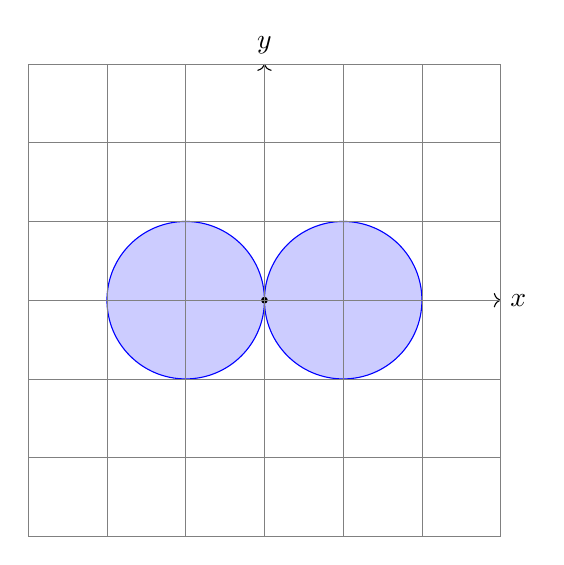
\begin{tikzpicture}
    % Draw the x and y axes
    \draw[->] (-3,0) -- (3,0) node[right] {$x$};
    \draw[->] (0,-3) -- (0,3) node[above] {$y$};
    
    % Shade and draw the first circle centered at (1,0) with radius 1
    \filldraw[fill=blue!20, draw=blue] (1,0) circle (1);
    
    % Shade and draw the second circle centered at (-1,0) with radius 1
    \filldraw[fill=blue!20, draw=blue] (-1,0) circle (1);
    
    % Mark the intersection point at the origin
    \filldraw (0,0) circle (1pt);
    
    % Add grid lines for better visualization (optional)
    \draw[step=1cm, gray, very thin] (-3,-3) grid (3,3);

\end{tikzpicture}\] Consider the union of two balls who intersect at the origin. Evidently, each ball is connected since they are path connected. The union of connected sets sharing a common point is connected (Theorem in book). Thus, the union is connected. Consider that the interior of the union does not contain the origin since any ball around the origin contains points in the plane not in either ball. Thus, we can express the interior of the union as two open balls which are disjoint and nonempty, and thus the interior of the union is disconnected. 
\end{solution}

\newpage
\section*{Problem 7}
\begin{problem}
    A function $f: (a,b) \to \bbR$ satisfies a $\alpha-$H\"{o}lder condition of order $\alpha$ if $\alpha>0,$ $H$ is a constant, and for all $u,x\in (a,b),$ we have 
    \[|f(u) - f(x)|\leq H|u-x|^\alpha\]
\end{problem}
\begin{enumerate}
    \item 
    \begin{problem}
        Prove that an $\alpha-$H\"{o}lder function defined on $(a,b)$ is uniformly continuous and infer that it extends uniquely to a continuous function defined on
        $[a, b].$ Is the extended function $\alpha-$H\"{o}lder?
    \end{problem}
    \begin{solution}
        Let $\epsilon>0.$ For all $u,x\in (a,b),$ there exists a $\delta = \min\{1, \frac{\epsilon}{|H| +1}\}$ such that if $|u-x|<\delta,$ we have that by the $\alpha-$H\"{o}lder condition,
        \[|f(u) - f(x)|\leq H|u-x|^\alpha < H|u-x|< |H| \frac{\epsilon}{|H|+1}<\epsilon.\]
        To extend this function to $[a,b],$ we need to define $f(a)$ and $f(b).$ To do this, let 
        \[f(a) = \lim_{x \to a^{+}}f(x),\qquad f(b) = \lim_{x \to b^{-}}f(x).\] Since limits are unique, then this is a unique extension on $[a,b].$ Continuity comes directly from the construction (See PSET 2). We claim that the extended function is $\alpha-$H\"{o}lder\\
        Let $x\in (a,b],$ we want to show that \[|f(a) - f(x)|\leq H|a-x|^\alpha.\] By continuity, for all $\epsilon>0,$ there exists some $\delta>0$ and $u\in (a,x)$ such that if $x-a<\delta,$ we have that $|f(a) - f(x)|<\epsilon.$ Thus,
        \begin{align*}
            |f(a) - f(x)|&\leq |f(a) - f(u)| + |f(u) - f(x)|\\
            &< \epsilon + H|u-x|^\alpha \\
            &\leq \epsilon + H|a-x|^\alpha
        \end{align*}
        Where the last inequality is justified since $|u-x|\leq |a-x|$ because $u\in (a,x).$ Thus, as $\epsilon\to 0,$ we have that $f$ is $\alpha-$H\"{o}lder continiuos at $a.$ A similar argument can be shown for $b.$
    \end{solution}
    \item
    \begin{problem}
        What does $\alpha-$H\"{o}lder continuity mean when $\alpha =1$?
    \end{problem}
    \begin{solution}
        If $\alpha = 1,$ we have that for all $u,x\in (a,b),$
        \[|f(u) - f(x)|\leq H|u-x|,\] and thus $f$ satisfies a global Lipschitz condition. Specifically, if $f$ is differentiable, then $|f'(x)|\leq H$ for all $x\in (a,b).$ Thus, the derivative is bounded for all $x\in (a,b)$.  
    \end{solution} 
    \item 
    \begin{problem}
        Prove that $\alpha-$H\"{o}lder continuity when $\alpha>1$ implies that $f$ is constant.
    \end{problem}
    \begin{solution}
        Let $x\in (a,b).$ Because $f$ is $\alpha-$H\"{o}lder, then 
        \[|f(u) - f(x)|\leq H |u-x|^\alpha.\] Thus, 
        \[0\leq \left|\frac{f(u) - f(x)}{u-x}\right|\leq H |u-x|^{\alpha - 1}\]
        Because $\alpha >1,$ then $|u-x|^{\alpha -1}$ is a well defined denominator. Consider that by continuity:
        \[\lim_{u\to x} (0) = 0,\qquad H\lim_{u\to x}|u-x|^{\alpha -1} = H(0) = 0,\] where the second limit comes from the fact that for $u$ close to $x,$ because $\alpha -1>0,$ we have that $|u-x|>|u-x|^{\alpha-1}.$ Thus, by the squeeze theorem, we have that 
        \[\lim_{u\to x}\left | \frac{f(u) - f(x)}{u-x}\right | =|f'(x)| =  0\] 
        It suffices to show that if $f'(x) = 0$ for any $x\in (a,b),$ we have that $f$ is constant. Let $y<x\in (a,b)$  By mean value theorem, we have that $f(y) - f(x) = f'(\lambda)(x-a) = 0,$ and thus $f(y)= f(x).$ 
    \end{solution}
\end{enumerate}

\newpage
\section*{Problem 8}
\begin{problem}
    For each $r \geq 1$, find a function that is $C^r$ but not $C^{r+1}$.
\end{problem}
\begin{solution}
Let $f_r: \bbR \to \bbR$ be defined by $f_r(x) = x^r|x|.$ We claim that $f_r$ is $C^r$ but not $C^{r+1}.$ We proceed by induction on $\bbN$ over the variable $r.$
\begin{enumerate}
    \item For $r = 1,$ we have that $f_1(x) = x|x|.$ We claim that $f'(x) = 2|x|.$ To see this, let $x>0,$ then $f_1'(x) = 2x.$ If $x<0,$ then $f_1'(x) = -2x.$ If $x = 0,$ then $f_1'(0) = 0.$ Thus, $f_1'(x) = 2|x|,$ which is continuous everywhere. Evidently, $f_1''(x)$ is not differentiable at $x=0.$ 
    \item Assume $f_r(x) = x^r|x|.$ is $C^r.$ Note that by similar work done above, $f_r^{(r)}(x) = r!|x|.$ Also assume that $f_r(x)$ is not $C^{r+1}$
    \item We claim that $f_{r+1}(x) = x^{(r+1)}|x|$ is $C^{r+1}.$ We have that, $f_{r+1}^{(r+1)}(x) = (r+1)!|x| = r!|x| + (r+1)|x|,$ which is continuous by hypothesis. Evidently, since $(r+1)|x|$ is not differentiable, we have that $f_{r+1}^{(r+2)}(x)$ is not continuous at $x=0$, and thus $f_{r+1}\notin C^{r+1}.$
\end{enumerate}
\end{solution}






























































\end{document}